\section{Learning the weight sharing scheme}

\subsection{Training settings}

The proposed formulation allows to learn both $S$ and $W$. We perform the two jointly. Learning $W$ amounts to learning weights as in regular CNNs, whereas learning $S$ amounts to learning how these weights are tied over the receptive fields. We also experiment a fine-tuning step, which consists in freezing $S$ in the last epochs. Indeed, when a weight sharing scheme can be decided directly from the underlying structure, it is not necessary to train $S$.

Because of our inspiration from CNNs, we propose constraints on the parameters of $S$. Namely, we impose them to be between 0 and 1, and to sum to 1 along the third dimension. Therefore, the vectors on the third rank of $S$ can be interpreted as performing a weighted average of the parameters in $W$.

We test two types of initialization for $S$. The first one consists in distributing one-hot-bit vectors along the third rank. We impose that for each receptive field, a particular one-hot-bit vector can only be distributed at most once more than any other. We refer to it as one-hot-bit initialization. The second one consists in using a uniform random distribution with limits as described in \cite{glorot2010understanding}.

\subsection{Discussion}

\todo{}

\subsection{Experiments with grid graphs}

Here we use models composed of a single receptive graph (or convolutional) layer made of 50 feature maps, without pooling, followed by a fully connected layer of 300 neurons, and terminated by a softmax layer of 10 neurons. Rectified Linear Units~\cite{glorot2011deep} are used for the activations and a dropout~\cite{srivastava2014dropout} of 0.5 is applied on the fully-connected layer. Input layers are regularized by a factor weight of $10^{-5}$~\cite{ng2004feature}. We optimize with ADAM~\cite{kingma2014adam} up to 100 epochs and fine-tune (while $S$ is frozen) for up to 50 additional epochs.

We consider a grid graph that connects each pixel to itself and its 4 nearest neighbors (or less on the borders). We also use the square of this graph (pixels are connected to their 13 nearest neighbors, including themselves), the cube of this graph (25 nearest neighbors), up to 10 powers (211 nearest neighbors).
Here we use one-hot-bit initialization. We test the model under two setups: either the ordering of the node is unknown, and then the one-hot-bit vectors are distributed randomly and modified upon training ; either an ordering of the node is known, and then the one-hot-bit vectors are distributed in a circulant fashion in the third rank of $S$ which is freezed in this state. We use the number of nearest neighbors as for the dimension of the third rank of $S$.
We also compare with a convolutional layer of size 5x5, thus containing as many weights as the cube of the grid graph. Table~\ref{toy} summarizes the obtained results. The ordering is unknown for the first result given, and known for the second result between parenthesis.

\begin{table}[H]
  \caption{Error rates on powers of the grid graphs on MNIST.}
  \begin{center}
    \bgroup
    \def\arraystretch{1.5}%  1 is the default, change whatever you need
    \begin{tabular}{|c|c|c|c|}
      \hline
      Conv5x5 & Grid$^1$ & Grid$^2$ & Grid$^3$\\
      \hline
      (0.87\%) & 1.24\% (1.21\%) & 1.02\% (0.91\%) & 0.93\% (0.91\%)\\
      \hline
      \hline
      Grid$^4$ & Grid$^5$ & Grid$^6$ & Grid$^{10}$\\
      \hline
      0.90\% (0.87\%) & 0.93\% (0.80\%) & 1.00\% (0.74\%) & 0.93\% (0.84\%)\\
      \hline
    \end{tabular}
    \egroup
  \end{center}
  \label{toy}
\end{table}

We observe that even without knowledge of the underlying euclidean structure, receptive grid graph layers obtain comparable performances as convolutional ones, and when the ordering is known, they match convolutions. We also noticed that after training, even though the one-hot-bit vectors used for initialization had changed  to floating point values, their most significant dimension was always the same. That suggests there is room to improve the initialization and the optimization.

In Figure~\ref{functionofepoch}, we plot the test error rate for various normalizations when using the square of the grid graph, as a function of the number of epochs of training. We observe that they have little influence on the performance and sometimes improve it a bit. Thus, we use them as optional hyperparameters.

\begin{figure}[H]
  \begin{center}
    % GNUPLOT: LaTeX picture with Postscript
\begingroup
  \makeatletter
  \providecommand\color[2][]{%
    \GenericError{(gnuplot) \space\space\space\@spaces}{%
      Package color not loaded in conjunction with
      terminal option `colourtext'%
    }{See the gnuplot documentation for explanation.%
    }{Either use 'blacktext' in gnuplot or load the package
      color.sty in LaTeX.}%
    \renewcommand\color[2][]{}%
  }%
  \providecommand\includegraphics[2][]{%
    \GenericError{(gnuplot) \space\space\space\@spaces}{%
      Package graphicx or graphics not loaded%
    }{See the gnuplot documentation for explanation.%
    }{The gnuplot epslatex terminal needs graphicx.sty or graphics.sty.}%
    \renewcommand\includegraphics[2][]{}%
  }%
  \providecommand\rotatebox[2]{#2}%
  \@ifundefined{ifGPcolor}{%
    \newif\ifGPcolor
    \GPcolortrue
  }{}%
  \@ifundefined{ifGPblacktext}{%
    \newif\ifGPblacktext
    \GPblacktextfalse
  }{}%
  % define a \g@addto@macro without @ in the name:
  \let\gplgaddtomacro\g@addto@macro
  % define empty templates for all commands taking text:
  \gdef\gplbacktext{}%
  \gdef\gplfronttext{}%
  \makeatother
  \ifGPblacktext
    % no textcolor at all
    \def\colorrgb#1{}%
    \def\colorgray#1{}%
  \else
    % gray or color?
    \ifGPcolor
      \def\colorrgb#1{\color[rgb]{#1}}%
      \def\colorgray#1{\color[gray]{#1}}%
      \expandafter\def\csname LTw\endcsname{\color{white}}%
      \expandafter\def\csname LTb\endcsname{\color{black}}%
      \expandafter\def\csname LTa\endcsname{\color{black}}%
      \expandafter\def\csname LT0\endcsname{\color[rgb]{1,0,0}}%
      \expandafter\def\csname LT1\endcsname{\color[rgb]{0,1,0}}%
      \expandafter\def\csname LT2\endcsname{\color[rgb]{0,0,1}}%
      \expandafter\def\csname LT3\endcsname{\color[rgb]{1,0,1}}%
      \expandafter\def\csname LT4\endcsname{\color[rgb]{0,1,1}}%
      \expandafter\def\csname LT5\endcsname{\color[rgb]{1,1,0}}%
      \expandafter\def\csname LT6\endcsname{\color[rgb]{0,0,0}}%
      \expandafter\def\csname LT7\endcsname{\color[rgb]{1,0.3,0}}%
      \expandafter\def\csname LT8\endcsname{\color[rgb]{0.5,0.5,0.5}}%
    \else
      % gray
      \def\colorrgb#1{\color{black}}%
      \def\colorgray#1{\color[gray]{#1}}%
      \expandafter\def\csname LTw\endcsname{\color{white}}%
      \expandafter\def\csname LTb\endcsname{\color{black}}%
      \expandafter\def\csname LTa\endcsname{\color{black}}%
      \expandafter\def\csname LT0\endcsname{\color{black}}%
      \expandafter\def\csname LT1\endcsname{\color{black}}%
      \expandafter\def\csname LT2\endcsname{\color{black}}%
      \expandafter\def\csname LT3\endcsname{\color{black}}%
      \expandafter\def\csname LT4\endcsname{\color{black}}%
      \expandafter\def\csname LT5\endcsname{\color{black}}%
      \expandafter\def\csname LT6\endcsname{\color{black}}%
      \expandafter\def\csname LT7\endcsname{\color{black}}%
      \expandafter\def\csname LT8\endcsname{\color{black}}%
    \fi
  \fi
    \setlength{\unitlength}{0.0500bp}%
    \ifx\gptboxheight\undefined%
      \newlength{\gptboxheight}%
      \newlength{\gptboxwidth}%
      \newsavebox{\gptboxtext}%
    \fi%
    \setlength{\fboxrule}{0.5pt}%
    \setlength{\fboxsep}{1pt}%
\begin{picture}(5040.00,3528.00)%
    \gplgaddtomacro\gplbacktext{%
      \colorrgb{0.38,0.38,0.38}%
      \put(946,751){\makebox(0,0)[r]{\strut{}$0.01$}}%
      \colorrgb{0.38,0.38,0.38}%
      \put(946,3263){\makebox(0,0)[r]{\strut{}$0.1$}}%
      \colorrgb{0.38,0.38,0.38}%
      \put(1125,484){\makebox(0,0){\strut{}$0$}}%
      \colorrgb{0.38,0.38,0.38}%
      \put(1829,484){\makebox(0,0){\strut{}$20$}}%
      \colorrgb{0.38,0.38,0.38}%
      \put(2532,484){\makebox(0,0){\strut{}$40$}}%
      \colorrgb{0.38,0.38,0.38}%
      \put(3236,484){\makebox(0,0){\strut{}$60$}}%
      \colorrgb{0.38,0.38,0.38}%
      \put(3939,484){\makebox(0,0){\strut{}$80$}}%
      \colorrgb{0.38,0.38,0.38}%
      \put(4643,484){\makebox(0,0){\strut{}$100$}}%
    }%
    \gplgaddtomacro\gplfronttext{%
      \csname LTb\endcsname%
      \put(176,2007){\rotatebox{-270}{\makebox(0,0){\strut{}Test error rate}}}%
      \put(2884,154){\makebox(0,0){\strut{}Epoch}}%
      \csname LTb\endcsname%
      \put(3656,3090){\makebox(0,0)[r]{\strut{}l2}}%
      \csname LTb\endcsname%
      \put(3656,2870){\makebox(0,0)[r]{\strut{}l2 + Pos}}%
      \csname LTb\endcsname%
      \put(3656,2650){\makebox(0,0)[r]{\strut{}None}}%
      \csname LTb\endcsname%
      \put(3656,2430){\makebox(0,0)[r]{\strut{}Norm + Pos}}%
      \csname LTb\endcsname%
      \put(3656,2210){\makebox(0,0)[r]{\strut{}l2 + Pos + Norm}}%
    }%
    \gplbacktext
    \put(0,0){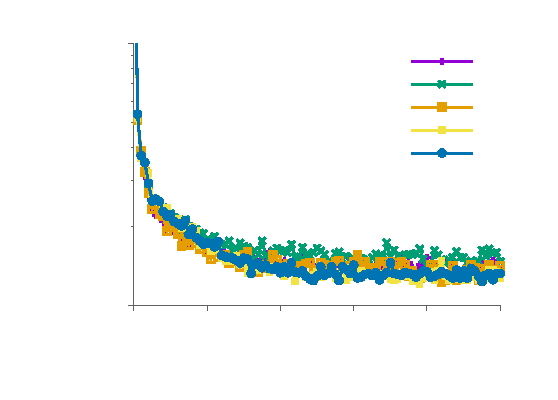
\includegraphics{chapter3/functionofepoch}}%
    \gplfronttext
  \end{picture}%
\endgroup

  \end{center}
  \caption{Evolution of the test error rate when learning MNIST using the square of a grid graph and for various normalizations, as a function of the epoch of training. The legend reads: ``l2'' means $\ell_2$ normalization of weights is used (with weights $10^{-5}$), ``Pos'' means parameters in $S$ are forced to being positive, and ``Norm'' means that the $\ell_1$ norm of each vector in the third dimension of $S$ is forced to 1.}
  \label{functionofepoch}
\end{figure}

\subsection{Experiments with covariance graphs}

We use a thresholded covariance matrix obtained by using all the training examples. We choose the threshold so that the number of remaining edges corresponds to a certain density $p$ (5x5 convolutions correspond approximately to a density of $p=3\%$). We also infer a graph based on the $k$ nearest neighbors of the inverse of the values of this covariance matrix ($k$-NN). The latter two are using no prior about the signal underlying structure. The pixels of the input images are shuffled and the same re-ordering of the pixels is used for every image. Dimension of the third rank of $S$ is chosen equal to $k$ and its weights are initialized random uniformly~\cite{glorot2010understanding}.
 The receptive graph layers are also compared with models obtained when replacing the first layer by a fully connected or convolutional one. Architecture used is the same as in the previous section. Results are reported on table~\ref{covar}.

\begin{table}[H]
  \caption{Error rates when topology is unknown on scrambled MNIST.}
  \begin{center}
    \bgroup
    \def\arraystretch{1.5}%  1 is the default, change whatever you need
    \begin{tabular}{|c|c|c|c|}
      \hline
      MLP & Conv5x5 & Thresholded ($p=3\%$) & $k$-NN ($k=25$)\\
      \hline
      1.44\% & 1.39\% & 1.06\% & 0.96\%\\
      \hline
    \end{tabular}
    \egroup
  \end{center}
  \label{covar}
  \end{table}

We observe that the receptive graph layers outperforms the CNN and the MLP on scrambled MNIST. This is remarkable because that suggests it has been able to exploit information about the underlying structure thanks to its graph.

\subsection{Improving $S$ for standard convolutions}

On Cifar10, we made experiments on shallow CNN architectures and replaced convolutions by receptive graphs. We report results on a variant of AlexNet~\cite{krizhevsky2012imagenet} using little distortion on the input that we borrowed from a tutorial of tensorflow~\cite{tensorflow2015-whitepaper}.
%On Cifar10, we use a variant of the AlexNet architecture applied on inputs with little distortion~\cite{krizhevsky2012imagenet}, borrowed from a tutorial of tensorflow~\cite{tensorflow2015-whitepaper}.
It is composed of two 5x5 convolutional layers of 64 feature maps, with max pooling and local response normalization, followed by two fully connected layers of 384 and 192 neurons.
%We switched each convolutional layer with receptive graph layers, but kept the pooling ones.
We compare two different graph supports: the one obtained by using the underlying graph of a regular 5x5 convolution, and the support of the square of the grid graph. Optimization is done with stochastic gradient descent on 375 epochs where $S$ is freezed on the 125 last ones. Circulant one-hot-bit intialization is used. These are weak classifiers for Cifar10 but they are enough to analyse the usefulness of the proposed layer. Exploring deeper architectures is left for further work. Experiments are run five times each. Means and standard deviations of accuracies are reported in table~\ref{cifar}. ``Pos'' means parameters in $S$ are forced to being positive, ``Norm'' means that the $\ell_1$ norm of each vector in the third dimension of $S$ is forced to 1, ``Both'' means both constraints are applied, and ``None'' means none are used.

\begin{table}[H]
  \caption{Accuracies (in \%) of shallow networks on CIFAR10.}
  \begin{center}
    \bgroup
    \def\arraystretch{1.5}%  1 is the default, change whatever you need
    \begin{tabular}{|c|c|c|c|c|c|c|}
      \hline
      Support & Learn $S$ & None & Pos & Norm & Both\\
      \hline
      \hline
      Conv5x5 & No & / & / & / & $86.8 \pm 0.2$\\
      \hline
      Conv5x5 & Yes & $87.4 \pm 0.1$ & $87.1 \pm 0.2$ & $87.1 \pm 0.2$ & $87.2 \pm 0.3$\\
      \hline
      Grid$^2$ & Yes & $87.3 \pm 0.2$ & $87.3 \pm 0.1$ & $87.5 \pm 0.1$ & $87.4 \pm 0.1$\\
      \hline
    \end{tabular}
    \egroup
  \end{center}
  \label{cifar}
\end{table}

The receptive graph layers are able to outperform the corresponding CNNs by a small amount in the tested configurations, opening the way for more complex architectures.

%idea
\todo{take S, and reuse it on resnet}

